% !TEX TS-program = pdflatex
% !TEX encoding = UTF-8 Unicode
% 
% This is a simple template for a LaTeX document using the "article" class.
% See "book", "report", "letter" for other types of document.
% 
\documentclass[11pt]{article} % use larger type; default would be 10pt
% 
% 
% 
%%% The "real" document content comes below...
\usepackage[utf8]{inputenc} % set input encoding (not needed with XeLaTeX)

%%% Examples of Article customizations
% These packages are optional, depending whether you want the features they provide.
% See the LaTeX Companion or other references for full information.

%%% PAGE DIMENSIONS
\usepackage{geometry} % to change the page dimensions
\geometry{a4paper} % or letterpaper (US) or a5paper or....
% \geometry{margin=2in} % for example, change the margins to 2 inches all round
% \geometry{landscape} % set up the page for landscape
%   read geometry.pdf for detailed page layout information

\usepackage{graphicx} % support the \includegraphics command and options

% \usepackage[parfill]{parskip} % Activate to begin paragraphs with an empty line rather than an indent

%%% PACKAGES
\usepackage{booktabs} % for much better looking tables
\usepackage{array} % for better arrays (eg matrices) in maths
\usepackage{paralist} % very flexible & customisable lists (eg. enumerate/itemize, etc.)
\usepackage{verbatim} % adds environment for commenting out blocks of text & for better verbatim
\usepackage{subfig} % make it possible to include more than one captioned figure/table in a single float
% These packages are all incorporated in the memoir class to one degree or another...

%%% HEADERS & FOOTERS
\usepackage{fancyhdr} % This should be set AFTER setting up the page geometry
\pagestyle{fancy} % options: empty , plain , fancy
\renewcommand{\headrulewidth}{0pt} % customise the layout...
\lhead{}\chead{}\rhead{}
\lfoot{}\cfoot{\thepage}\rfoot{}

%%% SECTION TITLE APPEARANCE
\usepackage{sectsty}
\allsectionsfont{\sffamily\mdseries\upshape} % (See the fntguide.pdf for font help)
% (This matches ConTeXt defaults)

%%% ToC (table of contents) APPEARANCE
\usepackage[nottoc,notlof,notlot]{tocbibind} % Put the bibliography in the ToC
\usepackage[titles,subfigure]{tocloft} % Alter the style of the Table of Contents
\renewcommand{\cftsecfont}{\rmfamily\mdseries\upshape}
\renewcommand{\cftsecpagefont}{\rmfamily\mdseries\upshape} % No bold!

%%% END Article customizations
\usepackage{xcolor}
\usepackage{tcolorbox}
\usepackage{lipsum}  % 示例文本
\usepackage{mdframed}

\usepackage{tikz}

% 
\title{Introduction to Math for DS Group Mini-project}
\author{IMDS Group 24 \\ Zehao Qian, Chloe Mendez, Mohammad Jamshaid Iqbal}
\begin{document}
% 
% 
% 
% Cover for the Project
% 
\begin{titlepage}
    \centering
    \vspace*{\fill}
    \vspace*{1cm}
    % \newline
    % \fontsize{12}{13}
    \textbf{\fontsize{17.28}{18}\selectfont Introduction to Math for DS Group Mini-project} \\
    \vspace{0.5cm}
    \fontsize{14}{16}\selectfont{Analysis of factors affecting Premier League match results} \\
    \vspace{1.5cm}
    \textbf{IMDS Group 24}
    \vfill
    % 
    % A thesis presented for the degree of \\ Doctor of Philosophy \\
    Zehao Qian, Chloe Mendez, Mohammad Jamshaid Iqbal \\
    \vspace{0.9cm}
    % "The mind prevails over matter,\\ transcending the ordinary to reach the divine."
    % 
    \vspace{0.9cm}
    \vspace{0.9cm}
    % \vspace{0.9cm}
    % 添加封面图片
    % 
\includegraphics[width=0.7\textwidth]{pic/cover_pic.tex}
    


\tikzset{every picture/.style={line width=0.75pt}} %set default line width to 0.75pt        

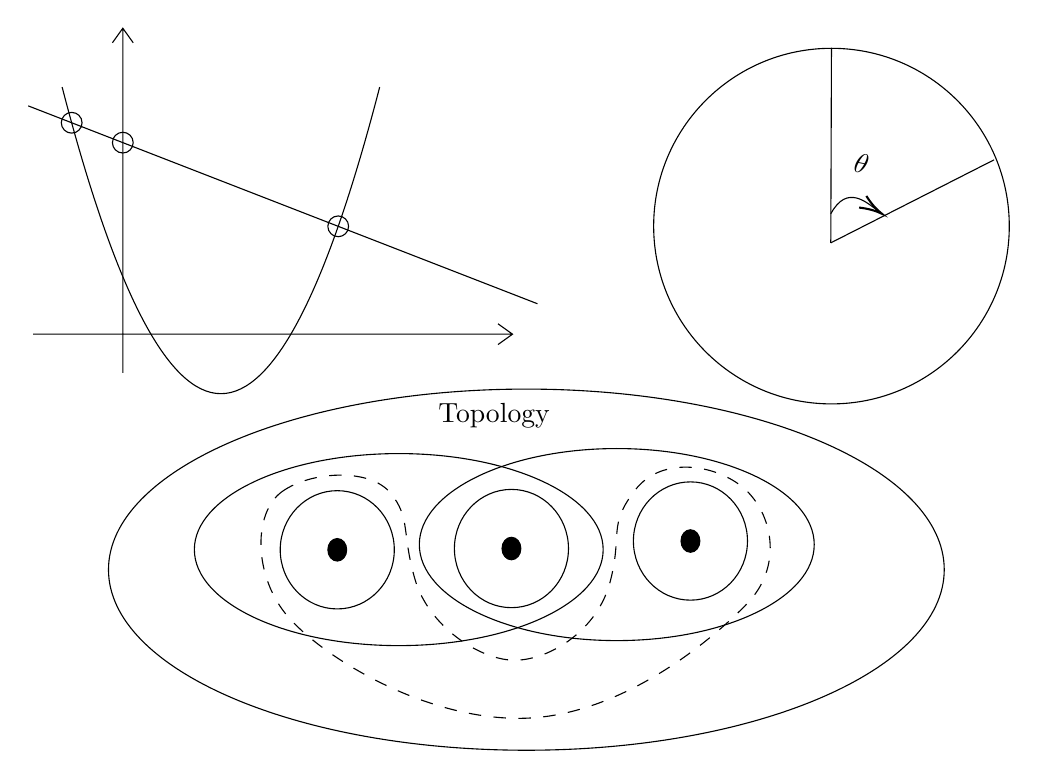
\begin{tikzpicture}[x=0.75pt,y=0.75pt,yscale=-1,xscale=1]
    %uncomment if require: \path (0,365); %set diagram left start at 0, and has height of 365

    %Shape: Axis 2D [id:dp3330650107827038] 
    \draw  (95.33,153.74) -- (326.33,153.74)(138.57,6.33) -- (138.57,172.41) (319.33,148.74) -- (326.33,153.74) -- (319.33,158.74) (133.57,13.33) -- (138.57,6.33) -- (143.57,13.33)  ;
    %Shape: Parabola [id:dp6747224874888704] 
    \draw   (109.33,34.67) .. controls (160.33,231.65) and (211.33,231.65) .. (262.33,34.67) ;
    %Straight Lines [id:da4045208158970277] 
    \draw    (93,43.74) -- (338.33,139.07) ;
    %Shape: Circle [id:dp9495260244967654] 
    \draw   (394.33,101.67) .. controls (394.33,54.35) and (432.69,16) .. (480,16) .. controls (527.31,16) and (565.67,54.35) .. (565.67,101.67) .. controls (565.67,148.98) and (527.31,187.33) .. (480,187.33) .. controls (432.69,187.33) and (394.33,148.98) .. (394.33,101.67) -- cycle ;
    %Straight Lines [id:da6440917457226727] 
    \draw    (480,16) -- (479.67,109.74) ;
    %Straight Lines [id:da2506243181764847] 
    \draw    (558.33,69.74) -- (479.67,109.74) ;
    %Curve Lines [id:da36631824919286937] 
    \draw    (479.67,95.74) .. controls (487.55,81.18) and (497.1,90.36) .. (502.77,94.64) ;
    \draw [shift={(504.33,95.74)}, rotate = 212.01] [color={rgb, 255:red, 0; green, 0; blue, 0 }  ][line width=0.75]    (10.93,-3.29) .. controls (6.95,-1.4) and (3.31,-0.3) .. (0,0) .. controls (3.31,0.3) and (6.95,1.4) .. (10.93,3.29)   ;
    %Shape: Ellipse [id:dp9329672718104849] 
    \draw   (131.67,267.19) .. controls (131.67,219.14) and (221.81,180.19) .. (333,180.19) .. controls (444.19,180.19) and (534.33,219.14) .. (534.33,267.19) .. controls (534.33,315.24) and (444.19,354.19) .. (333,354.19) .. controls (221.81,354.19) and (131.67,315.24) .. (131.67,267.19) -- cycle ;
    %Shape: Ellipse [id:dp9998724111128214] 
    \draw   (173.04,257.52) .. controls (173.04,231.97) and (217.13,211.26) .. (271.52,211.26) .. controls (325.91,211.26) and (370,231.97) .. (370,257.52) .. controls (370,283.08) and (325.91,303.79) .. (271.52,303.79) .. controls (217.13,303.79) and (173.04,283.08) .. (173.04,257.52) -- cycle ;
    %Shape: Ellipse [id:dp6415322670258081] 
    \draw   (281.43,255.11) .. controls (281.43,229.56) and (324.02,208.84) .. (376.56,208.84) .. controls (429.1,208.84) and (471.69,229.56) .. (471.69,255.11) .. controls (471.69,280.66) and (429.1,301.37) .. (376.56,301.37) .. controls (324.02,301.37) and (281.43,280.66) .. (281.43,255.11) -- cycle ;
    %Shape: Ellipse [id:dp6607583700307356] 
    \draw   (214.41,257.62) .. controls (214.41,241.88) and (226.72,229.13) .. (241.89,229.13) .. controls (257.07,229.13) and (269.37,241.88) .. (269.37,257.62) .. controls (269.37,273.35) and (257.07,286.11) .. (241.89,286.11) .. controls (226.72,286.11) and (214.41,273.35) .. (214.41,257.62) -- cycle ;
    %Shape: Ellipse [id:dp7853319365959068] 
    \draw   (298.33,257.01) .. controls (298.33,241.28) and (310.63,228.52) .. (325.81,228.52) .. controls (340.98,228.52) and (353.29,241.28) .. (353.29,257.01) .. controls (353.29,272.75) and (340.98,285.5) .. (325.81,285.5) .. controls (310.63,285.5) and (298.33,272.75) .. (298.33,257.01) -- cycle ;
    %Shape: Ellipse [id:dp5078229765284272] 
    \draw   (384.57,253.39) .. controls (384.57,237.65) and (396.87,224.9) .. (412.05,224.9) .. controls (427.23,224.9) and (439.53,237.65) .. (439.53,253.39) .. controls (439.53,269.12) and (427.23,281.88) .. (412.05,281.88) .. controls (396.87,281.88) and (384.57,269.12) .. (384.57,253.39) -- cycle ;
    %Shape: Ellipse [id:dp47882141993434524] 
    \draw  [fill={rgb, 255:red, 0; green, 0; blue, 0 }  ,fill opacity=1 ] (407.51,253.39) .. controls (407.51,250.4) and (409.55,247.97) .. (412.05,247.97) .. controls (414.56,247.97) and (416.59,250.4) .. (416.59,253.39) .. controls (416.59,256.38) and (414.56,258.81) .. (412.05,258.81) .. controls (409.55,258.81) and (407.51,256.38) .. (407.51,253.39) -- cycle ;
    %Shape: Polygon Curved [id:ds8181656794178567] 
    \draw  [dash pattern={on 4.5pt off 4.5pt}] (215.43,229.48) .. controls (229.33,219.68) and (257.43,218.15) .. (267.43,230.15) .. controls (277.43,242.15) and (272.76,249.48) .. (279.43,272.15) .. controls (286.1,294.82) and (311.3,311.28) .. (328.1,310.82) .. controls (344.89,310.35) and (367.43,296.15) .. (373.43,272.82) .. controls (379.43,249.48) and (372.1,246.15) .. (385.43,228.82) .. controls (398.76,211.48) and (426.76,216.82) .. (439.43,229.48) .. controls (452.1,242.15) and (456.1,266.15) .. (439.43,283.48) .. controls (422.76,300.82) and (378.14,338.48) .. (330.1,338.82) .. controls (282.05,339.16) and (232.1,307.48) .. (216.76,288.15) .. controls (201.43,268.82) and (201.52,239.29) .. (215.43,229.48) -- cycle ;
    %Shape: Ellipse [id:dp26952850031511955] 
    \draw  [fill={rgb, 255:red, 0; green, 0; blue, 0 }  ,fill opacity=1 ] (321.27,257.01) .. controls (321.27,254.02) and (323.3,251.59) .. (325.81,251.59) .. controls (328.31,251.59) and (330.34,254.02) .. (330.34,257.01) .. controls (330.34,260.01) and (328.31,262.43) .. (325.81,262.43) .. controls (323.3,262.43) and (321.27,260.01) .. (321.27,257.01) -- cycle ;
    %Shape: Ellipse [id:dp7070111192051278] 
    \draw  [fill={rgb, 255:red, 0; green, 0; blue, 0 }  ,fill opacity=1 ] (237.36,257.62) .. controls (237.36,254.62) and (239.39,252.2) .. (241.89,252.2) .. controls (244.4,252.2) and (246.43,254.62) .. (246.43,257.62) .. controls (246.43,260.61) and (244.4,263.04) .. (241.89,263.04) .. controls (239.39,263.04) and (237.36,260.61) .. (237.36,257.62) -- cycle ;

    % Text Node
    \draw (491.5,64.99) node [anchor=north west][inner sep=0.75pt]  [rotate=-12,xslant=0.03]  {$\theta $};
    % Text Node
    \draw (289.33,185.63) node [anchor=north west][inner sep=0.75pt]   [align=left] {Topology};

    \draw   (138.57, 61.45) circle [x radius= 5, y radius= 5]   ;
    \draw   (242.35, 101.77) circle [x radius= 5, y radius= 5]   ;
    \draw   (113.93, 51.87) circle [x radius= 5, y radius= 5]   ;
\end{tikzpicture}
    % 
    \vspace*{\fill}
\end{titlepage}
% 
% 
% 
% 
% 
\maketitle
% 
% 
% 
% 
\tableofcontents
% 
% 
% 
% 
% 
% 
\newpage
\section{Introduction}
% 
% 
\paragraph{The English Premier League is a ranking from one to twenty of the teams who won the most matches over the season. We are investigating the variables which factor into the ranking of the premier league; however, our dataset is fairly limited. We are examining historical data from previous seasons consisting of: the games won, lost and drawn by each team as well as the total number of goals for and against their team, and the goal difference. Ideally, we would analyse a dataset which featured variables not directly related to the ranking. In an attempt to enrich our dataset we performed the Fourier Transformation on the historical data from time domain to frequency domain. Time Domain feature extraction will allow us to examine the Time Domain evolution of the data. By analysing the time variability of metrics such as points, goals scored, goals conceded, etc., we hope to discover time-related patterns, such as seasonal changes or performance trends over a specific period. Of course, the most direct relationship is between the number of games won and the teams' placement on the league table, because this is how the table is curated. However, we did find some less obvious correlation; the teams' consistency in performance, as measured by a balanced distribution of wins, draws, and losses, is associated with a higher league position.  To test this hypothesis, we have made use of Principal Component Analysis (PCA), to find the most significant components, and the Entropy method (Entropy Weighting), with the intention of finding the overall weighting of the team's performance. With the goal of establishing that teams with a consistent performance history over the seasons is likely to allow them to maintain their competitive positions. PCA allows us to establish which were the most significant factors in achieving first place on the premier league table. This is appropriate for our dataset because our dataset's multicollinearity is very high, so we are using PCA to eliminate this issue. }
% 
% 
% 
% 
% 
\newpage
\section{Model Assumptions}
% 
% 
% 
\subsection{Performance Assumptions (Correlation Analysis)}
\begin{itemize}
    \item  The number of wins positively correlates with the final league standing.
    \item  Teams with a higher goal difference (GF - GA) tend to achieve higher league positions.
    \item Drawn matches have a minimal impact on final league standings.
    \item Teams with a higher number of goals scored (GF) are more likely to finish in the top positions.
    \item  The defensive performance, measured by goals against (GA), influences the team's final standing.
    \item  The number of points earned directly correlates with the team's final position in the league.
\end{itemize}
\subsection{Consistency Hypothesis (Principal Component Analysis)}
% 
% 
% 
% 
\begin{itemize}
    \item Consistency in performance, as measured by a balanced distribution of wins, draws, and losses, is associated with a higher league position.
\end{itemize}
\paragraph{PCA can help identify patterns and relationships among these variables, which can contribute to understanding the consistency in team performance.}
% 
% 
% 
% 
% 
\newpage
\section{Data}
% 
% 
% 
% 
% 
% 
% 
\newpage
\section{Methods}
% 
% 
\subsection{Data Feature Extraction with Fourier Transform}
% 
% 
% 
% 
% 
% 
% 
% 
\paragraph{Given that the Premier League data we crawled from the web is relatively limited, we are eager to enrich our feature set through feature extraction. To this end, we decided to treat historical match data as an information-rich signal and adopt time-domain and frequency-domain feature extraction methods to extract more key features from it, laying the foundation for a comprehensive analysis of the team's performance.}
% 
\paragraph{Therefore, in our research, we introduced Fourier transform, a powerful mathematical tool, to transform historical game data from time domain to frequency domain. Fourier transform is a method of converting time domain signals into frequency domain representation. Through this conversion, we are expected to reveal the underlying periodicity and frequency information in the data, providing strong support for deeper analysis and understanding.}
% 
% 
\paragraph{We will give the proof of the Fourier transform in the appendix section (\ref{sec:Fourier}). In its continuous form: $$ X(f) = \int_{-\infty}^{\infty} x(t) \cdot e^{-j2\pi ft} dt $$ Among them, X represents the frequency domain signal, and x represents the time domain signal. In the discrete form (because our data is discrete), we will use discrete Fourier transform methods such as fast Fourier transform (FFT) to calculate: $$ X(k) = \sum_{n=0}^{N-1} x(n) \cdot e^{-j2\pi kn/N} $$}
% 
% 
\paragraph{Time Domain feature extraction will allow us to delve into the Time Domain evolution of the data, revealing overall trends in the team over the past few years. By analyzing the time variability of metrics such as points, goals scored, goals conceded, etc., we can hopefully discover time-related patterns, such as seasonal changes or performance trends over a specific period.}
% 
\paragraph{At the same time, frequency domain feature extraction will help us understand the periodicity and frequency present in the data. This approach will help identify recurring seasonal patterns, allowing us to gain a more complete understanding of how a team's performance changes throughout the season. We will also explore whether specific events have a frequency-domain impact on team performance.}
% 
\paragraph{By converting historical match data into time and frequency domain features, we expect to be able to mine deeper information and provide a richer and more accurate feature set for our data-driven models to better interpret and predict Premier League matches. The team's performance. Here are the Time and Frequency Domain Features we will use:}
% 
% 
% 
% 
% 
% 
% 
% 
% 
\begin{table}[h]
    \centering
    \captionof{table}{Time Domain Features and Formulas}
    \begin{tabular}{|c|c|}
        \hline
        \textbf{Time Domain Feature} & \textbf{Formula for Time Domain Feature}                                                                                                         \\
        \hline
        Mean                         & $\text{mean} = \frac{1}{N} \sum_{i=1}^{N} x_i$                                                                                                   \\
        \hline
        Standard Deviation           & $\text{std\_dev} = \sqrt{\frac{1}{N} \sum_{i=1}^{N} (x_i - \text{mean})^2}$                                                                      \\
        \hline
        Root Mean Square (RMS)       & $\text{rms} = \sqrt{\frac{1}{N} \sum_{i=1}^{N} x_i^2}$                                                                                           \\
        \hline
        Skewness                     & $\text{skewness} = \frac{\frac{1}{N} \sum_{i=1}^{N} (x_i - \text{mean})^3}{\left(\frac{1}{N} \sum_{i=1}^{N} (x_i - \text{mean})^2\right)^{3/2}}$ \\
        \hline
        Kurtosis                     & $\text{kurtosis} = \frac{\frac{1}{N} \sum_{i=1}^{N} (x_i - \text{mean})^4}{\left(\frac{1}{N} \sum_{i=1}^{N} (x_i - \text{mean})^2\right)^2} - 3$ \\
        \hline
        Max Value                    & $\text{max\_value} = \max(\text{signal\_array})$                                                                                                 \\
        \hline
        Min Value                    & $\text{min\_value} = \min(\text{signal\_array})$                                                                                                 \\
        \hline
        Median                       & $\text{median} = \text{np.median}(\text{signal\_array})$                                                                                         \\
        \hline
        Zero Crossing Rate           & $\text{zero\_crossing\_rate} = \frac{\sum_{i=1}^{N-1} (\text{sign}(x_{i+1}) - \text{sign}(x_i)) \neq 0}{N}$                                      \\
        \hline
    \end{tabular}
\end{table}
% 
% 
% 
% 
% 
\begin{table}[h]
    \centering
    \captionof{table}{Frequency Domain Features and Formulas}
    \begin{tabular}{|c|c|}
        \hline
        \textbf{Frequency Domain Feature} & \textbf{Formula for Frequency Domain Feature}                                                                                            \\
        \hline
        Dominant Frequency                & $\text{dominant\_frequency} = \arg\max(\text{magnitude\_spectrum})$                                                                      \\
        \hline
        Max Frequency Magnitude           & $\text{max\_frequency\_magnitude} = \max(\text{magnitude\_spectrum})$                                                                    \\
        \hline
        Power Spectral Density            & $\text{power\_spectral\_density} = \frac{1}{N} \sum_{i=1}^{N} \text{magnitude\_spectrum}^2$                                              \\
        \hline
        Spectral Entropy                  & $\text{spectral\_entropy} = \text{entropy}(\text{magnitude\_spectrum})$                                                                  \\
        \hline
        Total Power                       & $\text{total\_power} = \sum_{i=1}^{N} x_i^2$                                                                                             \\
        \hline
        Centroid Frequency                & $\text{centroid\_frequency} = \frac{\sum_{i=1}^{N} i \cdot \text{magnitude\_spectrum}[i]}{\sum_{i=1}^{N} \text{magnitude\_spectrum}[i]}$ \\
        \hline
    \end{tabular}
\end{table}
% 
% 
% 
% 
\paragraph{We apply these formulas to our data (historical matches). 'Magnitude\_spectrum' is the magnitude of the spectrum calculated by Fourier transform.}
% 
% 
% 
% 
\subsection{Correlation Analysis}
% 
% 
% 
\paragraph{After feature extraction, we are preparing to conduct a thorough analysis of the relationship between various team indicators (MP, Win, Draw, Loss, GF, GA, GD and other features generated by last part) and the final score (Points) through correlation analysis. To choose an appropriate correlation analysis method, we will compare the characteristics of the Pearson correlation coefficient and the Spearman rank correlation coefficient, ultimately selecting the Spearman rank correlation coefficient for correlation analysis in English Premier League football.}
% 
% 
\begin{table}[h]
    \centering
    \caption{Characteristics of Pearson and Spearman Correlation Coefficients}
    % \begin{tabular}{|p{2.5cm}|p{5cm}|p{5cm}|}
    \begin{tabularx}{\textwidth}{|p{2.5cm}|X|X|}
        % \toprule
        \hline
        Characteristics     & Pearson Correlation Coefficient                                                                                       & Spearman Rank Correlation Coefficient                                                                                      \\
        % \midrule
        \hline
        Calculation         & $   r_{xy}=\frac{\sum{(X_i - \bar{X})(Y_i - \bar{Y})}}{\sqrt{\sum{(X_i - \bar{X})^2} \cdot \sum{(Y_i - \bar{Y})^2}}}$ & $ \rho = 1 - \frac{6\sum{d_i^2}}{n(n^2 - 1)}$                                                                              \\
        \hline
        Data Type           & Continuous variables                                                                                                  & Ordinal variables and non-linear relationships                                                                             \\
        \hline
        Linear Assumption   & Assumes a linear relationship between variables                                                                       & Does not make a specific linear assumption about the relationship                                                          \\
        \hline
        Applicability       & Works well when data is approximately normally distributed                                                            & Applicable to ordinal variables, non-linear relationships, or when data distribution does not follow a normal distribution \\
        \hline
        Outlier Sensitivity & Sensitive to outliers                                                                                                 & Relatively insensitive to outliers as it is based on ranks                                                                 \\
        \hline
        Interpretation      & Emphasizes the strength and direction of linear relationships                                                         & Focuses more on the ordinal relationship between variables                                                                 \\
        % \bottomrule
        \hline
    \end{tabularx}
\end{table}
% 
% 
% 
\paragraph{After comparing the above characteristics, we have decided to choose the Spearman rank correlation coefficient as our correlation analysis method. This is because in the context of English Premier League football matches, our data may not follow a normal distribution, and the Spearman rank correlation coefficient is more robust to non-linear relationships and ordinal variables, while being relatively insensitive to outliers. This makes it more suitable for our research purposes.}
% 
% 
\paragraph{In the report, we will use the Spearman rank correlation coefficient to explore the relationship between various team indicators and the final score, providing a more comprehensive understanding of the factors influencing different aspects of English Premier League football matches.}
% 
% 
% 
\subsection{Principal Component Analysis}
% 
% 
% 
% 
% 
\paragraph{Principal Component Analysis (PCA) is a technique for data dimensionality reduction and feature extraction. It achieves this by identifying the principal directions (principal components) in the data to reduce its dimensionality. Below are the detailed calculation steps for PCA, introducing an example dataset:}
% 
% 
% 
% 
\paragraph{Assume we have the following dataset:}
\begin{table}[h]
    \centering
    \caption{Example Dataset}
    \begin{tabular}{cccccccc}
        \toprule
        MP & Win & Draw & Loss & GF & GA & GD & Others \\
        \midrule
        38 & 27  & 6    & 5    & 80 & 22 & 58 & ...    \\
        38 & 25  & 10   & 3    & 65 & 26 & 39 & ...    \\
        38 & 24  & 11   & 3    & 74 & 31 & 43 & ...    \\
        38 & 21  & 13   & 4    & 67 & 28 & 39 & ...    \\
        38 & 19  & 8    & 11   & 55 & 33 & 22 & ...    \\
        \bottomrule
    \end{tabular}
\end{table}
% 
% 
% 
% 
% 
% 
\subsection*{Steps:}
% 
\subsubsection*{1. Standardize Data:}
% 
\paragraph{Standardize each feature, making its mean 0 and standard deviation 1. The standardization formula is:}
% 
\[ Z = \frac{(X - \bar{X})}{\sigma} \]
% 
\paragraph{where \(X\) is the original data, \(\bar{X}\) is the mean, and \(\sigma\) is the standard deviation. Applying this to the dataset yields the standardized data.}
% 
\subsubsection*{2. Compute Covariance Matrix:}
% 
\paragraph{The covariance matrix is the covariance matrix of the standardized data. The covariance matrix's formula is:}
% 
\[ \text{Cov}(X, Y) = \frac{\sum{(X_i - \bar{X})(Y_i - \bar{Y})}}{n-1} \]
% 
\paragraph{where \(X\) and \(Y\) are two features, \(\bar{X}\) and \(\bar{Y}\) are their means. After calculating the covariance matrix, we get:}
% 
% 
% 
% 
% 
% 
% 
% 
% 
\subsubsection*{3. Compute Eigenvalues and Eigenvectors:}
% 
\paragraph{Perform eigenvalue decomposition on the covariance matrix to obtain eigenvalues and their corresponding eigenvectors. Eigenvalues represent variance in the data, and eigenvectors are the directions of principal components.}
% 
\subsubsection*{4. Select Principal Components:}
% 
\paragraph{Based on the magnitude of eigenvalues, choose the number of principal components to retain. Typically, you might select components that capture a certain percentage of variance, such as 90\%.}
% 
\subsubsection*{5. Build Projection Matrix:}
% 
\paragraph{Compose a matrix with the selected eigenvectors as columns. This matrix serves as the projection matrix, mapping the original data into the new principal component space.}
% 
\subsubsection*{6. Project to New Principal Component Space:}
\paragraph{Multiply the standardized data by the projection matrix to obtain the reduced-dimensional data.}
% 
% 
% 
% \subsection{Comparison: Entropy Weight Method}
% 
% 
% 
% 
% 
\newpage
\section{Conclusions}
% 
% 
% 
% 
% 
% 
% 
\newpage
% 
% 
\appendix
% 
\section{A breif proof for Fourier Transform}\label{sec:Fourier}
% 
\paragraph{The continuous Fourier Transform of a function \( f(t) \) is given by:}
\[ F(\omega) = \int_{-\infty}^{\infty} f(t) \cdot e^{-i \omega t} \,dt \]
\paragraph{To prove this, we start with the Fourier series representation of a periodic function. Let \( T \) be the period of \( f(t) \). The Fourier series expansion is given by:}
% 
\[ f(t) = \sum_{n=-\infty}^{\infty} c_n e^{i \omega_n t} \]
% 
\paragraph{Here, \( c_n \) are the Fourier coefficients, and \( \omega_n = \frac{2\pi n}{T} \) are the angular frequencies.}
% 
\paragraph{Now, consider the limit as \( T \) approaches infinity, turning the sum into an integral:}
% 
\[ f(t) = \lim_{T \to \infty} \sum_{n=-\infty}^{\infty} c_n e^{i \omega_n t} \]
% 
\paragraph{This leads to the continuous Fourier Transform integral:}
% 
\[ F(\omega) = \lim_{T \to \infty} \int_{-\frac{T}{2}}^{\frac{T}{2}} f(t) e^{-i \omega t} \,dt \]
% 
\paragraph{As \( T \) approaches infinity, the limits of integration become \( -\infty \) to \( \infty \):}
% 
\[ F(\omega) = \lim_{T \to \infty} \int_{-\infty}^{\infty} f(t) e^{-i \omega t} \,dt \]
% 
\paragraph{This is essentially the definition of the continuous Fourier Transform. The limit is introduced to handle functions that are not strictly periodic.}
% 
\paragraph{The rigorous proof involves showing that this limit exists for a wide class of functions and exploring the convergence properties. It requires knowledge of mathematical analysis and complex analysis.}
% 
% 
% 
% 
% 
% 
\section{Data Set}
\paragraph{Due to the large number of datasets and the number of columns, we uploaded the data to GitHub, and below are links to the various datasets.}
\subsection{Data Original Source}
\paragraph{The data set we got from FootyStats.org and we saved them with csv format.}
\paragraph{\href{https://github.com/QianZeHao123/IMDS/tree/main/notes_and_assignments/group-project/src/Data}{Click the Hyperlink here and Review the orginal data set.}}
% 
% 
% 
\subsection{The processed dataset}
\paragraph{\href{https://github.com/QianZeHao123/IMDS/blob/main/notes_and_assignments/group-project/src/Results/2023_24_General.csv}{A data set for combining the 2023-24 season data and historical features.}}
% 
% 
\paragraph{\href{https://github.com/QianZeHao123/IMDS/blob/main/notes_and_assignments/group-project/src/Results/2023_24_Processed.csv}{Data set for caculating the Correlation between variables and Points}}
% 
% 
\paragraph{\href{https://github.com/QianZeHao123/IMDS/blob/main/notes_and_assignments/group-project/src/Results/2023_24_Processed_PCA.csv}{Data set for caculating PCA}}
% 
% 
\subsection{Dataset for Saving Results}
% 
% 
\paragraph{\href{https://github.com/QianZeHao123/IMDS/blob/main/notes_and_assignments/group-project/src/Results/Cor_result.csv}{Results about Correlation between variables and Points}}
% 
% 
\paragraph{\href{https://github.com/QianZeHao123/IMDS/blob/main/notes_and_assignments/group-project/src/Results/pca_result.csv}{Results about PCA}}
% 
% 
% 
% 
% 
% 
% 
% 
% 
% 
% 
% 
% 
% 
% 
% 
% 
% 
% 
% 
% 
\section{Premier League Data Fetch Scripts}\label{sec:GetData}
\begin{lstlisting}[style=pystyle]
from selenium import webdriver
from selenium.webdriver.common.by import By
import re
from selenium.webdriver.support.ui import WebDriverWait
# from selenium.webdriver.support.select import Select
from selenium.webdriver.support import expected_conditions as EC
import time
import csv

options = webdriver.EdgeOptions()
options.add_experimental_option("detach", True)
driver = webdriver.Edge()
driver.maximize_window()
driver.get('https://footystats.org/england/premier-league')

start_year = 2007
end_year = 2023
Years = [
    f'{year}/{str(year+1)[-2:]}' for year in range(start_year, end_year + 1)]
# year = '2022/23'


for year in Years:
    select = driver.find_element(By.CLASS_NAME, "drop-down-parent.fl.boldFont")
    select.click()
    time.sleep(2)
    # Replace 'your_data_hash_value' with the specific value you want to select
    # chooseSeason = driver.find_element(By.)
    # get element
    element = WebDriverWait(driver, 10).until(
        EC.element_to_be_clickable((By.LINK_TEXT, year))
    )
    element.click()
    time.sleep(2)
    # mp, win, draw, loss, gf, ga, gd
    # Find an element by its class (replace 'element_class' with the actual class of the element on the webpage)
    TEAMs = driver.find_elements(
        By.CLASS_NAME, 'bold.hover-modal-parent.hover-modal-ajax-team')
    MPs = driver.find_elements(By.CLASS_NAME, 'mp')
    WINs = driver.find_elements(By.CLASS_NAME, 'win')
    DRAWs = driver.find_elements(By.CLASS_NAME, 'draw')
    LOSSs = driver.find_elements(By.CLASS_NAME, 'loss')
    GFs = driver.find_elements(By.CLASS_NAME, 'gf')
    GAs = driver.find_elements(By.CLASS_NAME, 'ga')
    GDs = driver.find_elements(By.CLASS_NAME, 'gd')
    POINTs = driver.find_elements(By.CLASS_NAME, 'points.bold')
    # Get text content from the element
    team_list = []
    mp_list = []
    win_list = []
    draw_list = []
    loss_list = []
    gf_list = []
    ga_list = []
    gd_list = []
    point_list = []

    for team in TEAMs:
        text_content = team.text
        team_list.append(text_content)

    for mp in MPs:
        text_content = mp.text
        # Use regex to extract only numbers
        numbers = re.findall(r'\d+', text_content)
        # Concatenate the numbers if there are multiple matches
        valid_numbers = [int(num) for num in numbers if num]
        # Append the valid numbers to the list
        mp_list.extend(valid_numbers)

    for win in WINs:
        text_content = win.text
        # Use regex to extract only numbers
        numbers = re.findall(r'\d+', text_content)
        # Concatenate the numbers if there are multiple matches
        valid_numbers = [int(num) for num in numbers if num]
        # Append the valid numbers to the list
        win_list.extend(valid_numbers)

    for draw in DRAWs:
        text_content = draw.text
        # Use regex to extract only numbers
        numbers = re.findall(r'\d+', text_content)
        # Concatenate the numbers if there are multiple matches
        valid_numbers = [int(num) for num in numbers if num]
        # Append the valid numbers to the list
        draw_list.extend(valid_numbers)

    for loss in LOSSs:
        text_content = loss.text
        # Use regex to extract only numbers
        numbers = re.findall(r'\d+', text_content)
        # Concatenate the numbers if there are multiple matches
        valid_numbers = [int(num) for num in numbers if num]
        # Append the valid numbers to the list
        loss_list.extend(valid_numbers)

    for gf in GFs:
        text_content = gf.text
        # Use regex to extract only numbers
        numbers = re.findall(r'\d+', text_content)
        # Concatenate the numbers if there are multiple matches
        valid_numbers = [int(num) for num in numbers if num]
        # Append the valid numbers to the list
        gf_list.extend(valid_numbers)

    for ga in GAs:
        text_content = ga.text
        # Use regex to extract only numbers
        numbers = re.findall(r'\d+', text_content)
        # Concatenate the numbers if there are multiple matches
        valid_numbers = [int(num) for num in numbers if num]
        # Append the valid numbers to the list
        ga_list.extend(valid_numbers)

    for gd in GDs:
        text_content = gd.text
        # Use regex to extract only numbers
        numbers = re.findall(r'-?\d+', text_content)
        # Concatenate the numbers if there are multiple matches
        valid_numbers = [int(num) for num in numbers if num]
        # Append the valid numbers to the list
        gd_list.extend(valid_numbers)

    for point in POINTs:
        text_content = point.text
        # Use regex to extract only numbers
        numbers = re.findall(r'\d+', text_content)
        # Concatenate the numbers if there are multiple matches
        valid_numbers = [int(num) for num in numbers if num]
        # Append the valid numbers to the list
        point_list.extend(valid_numbers)

    # Print the list of extracted numbers
    print('TEAM List is:', team_list)
    print('MP List is:', mp_list)
    print('WIN List is:', win_list)
    print('DRAW List is:', draw_list)
    print('Loss List is:', loss_list)
    print('GF List is:', gf_list)
    print('GA List is:', ga_list)
    print('GD List is:', gd_list)
    print('POINT List is:', point_list)

    # CSV file
    year_file = year.replace('/', '_')
    csv_file_path = './' + 'Data/' + year_file + '.csv'

    # write data to csv
    with open(csv_file_path, mode='w', newline='', encoding='utf-8') as file:
        writer = csv.writer(file)

        # edit header
        header = ['Team', 'MP', 'Win', 'Draw',
                    'Loss', 'GF', 'GA', 'GD', 'Points']
        writer.writerow(header)

        # write data
        for i in range(len(team_list)):
            row = [team_list[i], mp_list[i], win_list[i], draw_list[i],
                    loss_list[i], gf_list[i], ga_list[i], gd_list[i], point_list[i]]
            writer.writerow(row)

    print(f'Data has been written to {csv_file_path}')

driver.quit()

\end{lstlisting}
% 
% 
% 
% 
\section{Feature Extract Function}\label{sec:FEF}
% 
% 
\subsection{extractFeatures.py}
\begin{lstlisting}[style=pystyle]
import pandas as pd
import numpy as np
from scipy.stats import skew, kurtosis
from scipy.fftpack import fft
from scipy.signal import find_peaks
from scipy.stats import entropy


def extract_features(signal):
    features = {}

    # Convert the column to numeric, handling non-numeric values
    signal_numeric = pd.to_numeric(signal, errors='coerce')

    # Replace or remove specific non-numeric values
    signal_numeric.replace('ALIGNED', np.nan, inplace=True)

    # Remove NaN values or use interpolation as needed
    signal_numeric.dropna(inplace=True)

    # Convert to NumPy array
    signal_array = signal_numeric.to_numpy()

    # Check if the array is not empty
    if len(signal_array) > 0:
        # Time-domain features
        features['mean'] = np.mean(signal_array)
        features['std_dev'] = np.std(signal_array)
        features['rms'] = np.sqrt(np.mean(np.square(signal_array)))
        features['skewness'] = skew(signal_array)
        features['kurtosis'] = kurtosis(signal_array)
        features['max_value'] = np.max(signal_array)
        features['min_value'] = np.min(signal_array)
        features['median'] = np.median(signal_array)
        features['iqr'] = np.percentile(
            signal_array, 75) - np.percentile(signal_array, 25)
        features['zero_crossing_rate'] = np.sum(
            np.diff(np.sign(signal_array)) != 0) / len(signal_array)

        # Frequency-domain features using FFT
        try:
            fft_result = fft(signal_array)
            magnitude_spectrum = np.abs(fft_result)

            features['dominant_frequency'] = np.argmax(magnitude_spectrum)
            features['max_frequency_magnitude'] = np.max(magnitude_spectrum)

            # Statistical measures
            # features['auto_correlation'] = np.correlate(
            #     signal_array, signal_array, mode='full')

            # Frequency-domain features
            features['power_spectral_density'] = np.mean(
                np.square(magnitude_spectrum))
            features['total_power'] = np.sum(np.square(signal_array))
            features['spectral_entropy'] = entropy(magnitude_spectrum)
            features['centroid_frequency'] = np.sum(np.arange(
                len(magnitude_spectrum)) * magnitude_spectrum) / np.sum(magnitude_spectrum)

            # Time-frequency features
            # Add your wavelet transform code here
            # Example using FFT for STFT
            # features['wavelet_coefficients'] = []
            # features['stft'] = np.abs(np.fft.fftshift(
            # np.fft.fft(signal_array)))

            # Other features
            # features['peaks_count'], _ = find_peaks(signal_array)

        except ValueError as e:
            print(f"Error in FFT calculation: {e}")

    return features
\end{lstlisting}
% 
% 
% 
% 
% 
% 
\subsection{Using Data Extraction Function}
% 
\begin{lstlisting}[style=pystyle]

import os
import pandas as pd
from extractFeatures import extract_features

# Folder path containing all CSV files
folder_path = "./Data"

# Target team
target_team = "Everton FC"
target_teams = ['Manchester City FC', 'Liverpool FC', 'Arsenal FC',
                'Tottenham Hotspur FC', 'Aston Villa FC',
                'Manchester United FC', 'Newcastle United FC',
                'Brighton & Hove Albion FC', 'West Ham United FC',
                'Chelsea FC', 'Brentford FC', 'Crystal Palace FC',
                'Wolverhampton Wanderers FC', 'Nottingham Forest FC',
                'Fulham FC', 'AFC Bournemouth', 'Luton Town FC',
                'Sheffield United FC', 'Everton FC', 'Burnley FC']
# List of all CSV file names
csv_files = [
    '2007_08.csv', '2008_09.csv', '2009_10.csv', '2010_11.csv',
    '2011_12.csv', '2012_13.csv', '2013_14.csv', '2014_15.csv',
    '2015_16.csv', '2016_17.csv', '2017_18.csv', '2018_19.csv',
    '2019_20.csv', '2020_21.csv', '2021_22.csv', '2022_23.csv'
]



def get_result_df(target_team):
    # Create an empty DataFrame to store the extracted data
    result_df = pd.DataFrame(
        columns=["File", "Team", "MP", "Win",
                    "Draw", "Loss", "GF", "GA",
                    "GD", "Points"]
    )
    # Loop through each CSV file
    for csv_file in csv_files:
        # Build the full path of the CSV file
        file_path = os.path.join(folder_path, csv_file)

        # Read the CSV file
        df = pd.read_csv(file_path)

        # Extract data for the target team
        team_data = df[df["Team"] == target_team]

        # If data for the target team is found, add it to the result DataFrame
        if not team_data.empty:
            # Use pd.concat to add the target team's data from the current file to the result DataFrame,
            # and add the file name column
            result_df = pd.concat(
                [result_df, team_data.assign(File=csv_file)], ignore_index=True)

    return result_df

# print(result_df)
# result_df.to_csv("output.csv", index=False)

selected_columns = ['Win','Draw','Loss','GF','GA','GD','Points']

dfs = []

for target_team in target_teams:
    result_df = get_result_df(target_team)


    features_dict = {}
    for column in selected_columns:
        selected_data = result_df[column]
        features_column = extract_features(selected_data)
        features_dict[column] = features_column

    # Flatten the nested structure and convert to a DataFrame
    flattened_features = {}
    for column, feature_dict in features_dict.items():
        for key, value in feature_dict.items():
            flattened_features[f'{column}_{key}'] = value

    flattened_df = pd.DataFrame([flattened_features])

    # Append the DataFrame to the list
    dfs.append(flattened_df)

# Concatenate all DataFrames into a single DataFrame

result_df = pd.concat(dfs, ignore_index=True)

df_23_24 = pd.read_csv('./Data/2023_24.csv')
result = pd.concat([df_23_24, result_df], axis=1)
# Export the result to a CSV file
result.to_csv("2023_24_General.csv", index=False)
\end{lstlisting}
% 
% 
% 
% 
% 
% 
% 
% 
% 
% 
% 
% 
% 
% 
% 
% 
% 
% 
\section{Correlation Calculating}\label{sec:CC}
% 
% 
% 
\begin{lstlisting}[style=pystyle]
# Import the pandas library
import pandas as pd

# Read the CSV file
# Replace '2023_24_Processed.csv' with the actual file name and path
df = pd.read_csv('./Results/2023_24_Processed.csv')

# Define the target column for Spearman correlation
target_column = 'Points'

# Calculate Spearman correlation between the target column and all other columns
correlation_result = df.corrwith(df[target_column], method='spearman')

# Create a DataFrame containing the correlation results
result_df = pd.DataFrame({
    'Positive Correlation': correlation_result[correlation_result > 0].sort_values(ascending=False),
    'Negative Correlation': correlation_result[correlation_result < 0].sort_values(ascending=True)
})

# Print the results
print(result_df)

# Save the results to a CSV file
result_df.to_csv('./Results/Cor_result.csv', index=True)

# Extract the variables with absolute correlation greater than 0.6
positive_correlation_list = correlation_result[(correlation_result > 0) & (correlation_result.abs() > 0.65)].sort_values(ascending=False)
negative_correlation_list = correlation_result[(correlation_result < 0) & (correlation_result.abs() > 0.65)].sort_values(ascending=True)

# Print the lists of variables with absolute correlation greater than 0.6
print(positive_correlation_list)
print(negative_correlation_list)

positive_correlation_list.to_csv('./Results/Positive_Cor_result.csv', index=True)
negative_correlation_list.to_csv('./Results/Negative_Cor_result.csv', index=True)


positive_correlation_variables = list(positive_correlation_list.index)
negative_correlation_variables = list(negative_correlation_list.index)


print(positive_correlation_variables)
print(negative_correlation_variables)
\end{lstlisting}
% 
% 
% 
% 
% 
% 
% 
% 
% 
% 
% 
% 
% 
% 
% 
% 
% 
% 
% 
% 
% 
% 
% 
% 
% 
\section{PCA Analysis Implementation}\label{sec:PCA}
% 
\begin{lstlisting}[style=pystyle]
# Import the pandas library
import pandas as pd
from sklearn.decomposition import PCA


# Read the CSV file
# Replace '2023_24_Processed.csv' with the actual file name and path
df = pd.read_csv('./Results/2023_24_Processed.csv')


select_col = ['Win', 'GD', 'GF', 'GF_max_value', 'GD_max_value', 'Points_rms',
                'GF_mean', 'Points_mean', 'GF_rms', 'Win_rms', 'GF_median', 'Points_max_value',
                'GD_mean', 'Win_max_value', 'GF_power_spectral_density', 'GF_total_power',
                'Win_mean', 'GF_max_frequency_magnitude', 'Points_power_spectral_density',
                'Points_max_frequency_magnitude', 'Points_total_power', 'Win_total_power',
                'Win_power_spectral_density', 'Points_median', 'GF_min_value', 'GF_std_dev',
                'Draw_centroid_frequency', 'Loss', 'GA', 'Loss_min_value', 'Loss_mean',
                'Loss_rms', 'Loss_median', 'Loss_max_value']


selected_columns = df[select_col]
selected_columns.to_csv('./Results/2023_24_Processed_PCA.csv', index=False)

pca = PCA()
pca_result = pca.fit_transform(selected_columns)

pca_df = pd.DataFrame(data=pca_result, columns=[
                        f'PC{i+1}' for i in range(pca_result.shape[1])])
# result_df = pd.concat([selected_columns.reset_index(drop=True), pca_df], axis=1)

# result_df.to_csv('./pca_result.csv', index=False)
pca_df.to_csv('./Results/pca_result.csv', index=False)

\end{lstlisting}
% 
% 
% 
% 
% 
\end{document}
% \input{example}
% \section{Problem}
% \paragraph{Looking to find out which team is more likely to win the league given their current form. The focus will be on the English Premier League and the target is that the model can be used for other leagues too.}
% \section{Variables}
% \paragraph{The variables that we will be taking in are the following:}
% % 
% % 
% % 
% \begin{enumerate}
%     \item The number of matches won by the nth game week, v1.
%     \item The number of matches lost by the nth game week, v2.
%     \item The number of matches drawn by the nth game week, v3.
%     \item The number of goals scored by the nth game week, v4.
%     \item The number of goals conceded by the nth game week, v5.
%     \item The number of points gained by the nth game week, v6.
%     \item The number of matches in the last 5 games, v7
% \end{enumerate}
% % 
% % 
% % 
% % 
% \section{Method}
% \paragraph{We will change these variables into a 7-dimensional vector:}
% $$ V = [v1, v2, v3, v4, v5, v6, v7] $$
% \subsection{METHOD 1}
% \paragraph{The first method that I can think of is using vector projection to see which team will be performing the best by the end of the season given current statistics.}
% % 
% % 
% \paragraph{We will then normalize the above vector for each team using the following formula:}
% % 
% % 
% \paragraph{This will help us to compare the team's performance with each other.
% We can then define a reference vector; a reference vector can be calculated using the performance of previous champions by the nth game week for the season they were championed it. If we have the data for the past 10 seasons, then we will have 10 reference vectors and we can take the average out for those reference vectors. Let's call this reference vector Vr.}
% \paragraph{Next, we will project each team's normalized vector onto the reference vector. This will give us how each team's performance is compared to an ideal performance.
% The team with the largest projection is the team that is most likely to win.}
% % 
% % 
% % 
% % 
% \subsection{METHOD 2}
% \paragraph{This vector is basically representing the team's performance till the nth game week. We can use this vector to predict team's performance for the remaining matches by applying linear transformation.}
% \paragraph{The linear transformation will basically transform the 7-dimensional vector to a 1-dimensional vector which will be the total number of points by the team.
% Fv : R7 -> R}
% \paragraph{The linear transformation F will take in the vector V which is the vector of the team's statistics in the nth game week and map it to the predicted point at the end of the season.}
% F(V) = wV + b
% \paragraph{w is the 7-dimensional weighted vector which is basically a weighted vector for each statistic. b is the scalar bias. Scalar bias is a systematic error in a model and the importance of scalar bias will be to make the value of the points closer to the accurate value.}
% \paragraph{To take out the weighted vector and scalar bias, we will use the data of previous seasons (we can use the data of 10 years) and then use gradient descent in Python. After inputting the historical data, we will be able to take out the weighted vectors and scalar bias which then can be applied to the formula above to take out the points.}
% % 
% % 
% % 
% % 
% % 
% % 
% % 
% % 
% % 
% \section{Limitations}
% % 
% % 
% \paragraph{The model just takes in the statistics such as wins till a certain game week, the number of goals scored, etc. as input. This might not be an accurate representation of the prediction for who will win the Premier League. This could be because there are other factors that can come into play such as the number of quality players bought by a team, the amount of money spent on transfers, the number of players injured during the season, the experience of managers, etc. There are many more factors that could affect a team's performance throughout the season, but our model uses the on-field statistics to predict who will win the league. A linear regression model can be used to check the accurate representation of who will win the league by using more data.}
% 
% 
% 
% 
% 
% 
% 
% 
% 
% \section{Data}
% \href{https://www.premierleague.com/tables}{https://www.premierleague.com/tables}
% 
% 
% 
% 
% \begin{lstlisting}[style=pystyle]
% import numpy as np
% # Define the matrices A and B
% A = np.array([
%     [1, 0, 4, 1],
%     [0, 2, 0, 2],
%     [6, 0, 3, 11]
% ])

% B = np.array([
%     [7, -1, 2],
%     [1, 1, 0],
%     [2, 0, 1]
% ])

% # Calculate the product of A and B
% AB_product = np.dot(A, B)
% AB_product    
% \end{lstlisting}
% 
% 
% 
% 
% \paragraph{\textcolor{red}{Return ValueError: shapes (3,4) and (3,3) not aligned: 4 (dim 1) != 3 (dim 0)}}
% 
% 
% \paragraph{\textbf{Analytics:} The product of two matrices AB is undefined if the number of columns in the first matrix A does not match the number of rows in the second matrix B. In this case, matrix A has 4 columns, while matrix B has 3 rows, so their product cannot be computed. Matrix multiplication requires that the number of columns in the first matrix be equal to the number of rows in the second matrix. If there's a third matrix C that should be involved to make the multiplication possible, please provide it, otherwise matrix A and B as given cannot be multiplied.}
% 
% 
% 
% 
% 
% 
% 
% 
% 
% 
% 
% 
% 
% 
% \section{Question 2}
% \paragraph{What is the dimension of the span of the vectors $(5,7,9,0)$, $(2,5,0,1)$, $(0,0,0,1)$ and $(7,12,9,3)$?}
% 
% 
% 
% 
% 
% 
% \subsection{AI Bot's Answer}
% \begin{mdframed}[
%         backgroundcolor=white,  % 背景颜色
%         linecolor=black,        % 边框颜色
%         leftmargin=5pt,         % 左边距
%         rightmargin=5pt,        % 右边距
%         linewidth=2pt           % 边框的宽度
%     ]
%     \paragraph{\textbf{ChatGPT}: To find the dimension of the span of the given vectors, we can create a matrix using these vectors as columns and then find the rank of the matrix.}
%     % 
%     \paragraph{The given vectors are:}
%     % 
%     \[
%         \begin{bmatrix}
%             5 \\
%             7 \\
%             9 \\
%             0
%         \end{bmatrix},
%         \begin{bmatrix}
%             2 \\
%             5 \\
%             0 \\
%             1
%         \end{bmatrix},
%         \begin{bmatrix}
%             0 \\
%             0 \\
%             0 \\
%             1
%         \end{bmatrix},
%         \begin{bmatrix}
%             7  \\
%             12 \\
%             9  \\
%             3
%         \end{bmatrix}
%     \]
%     % 
%     \paragraph{Let's create a matrix \(M\) using these vectors:}

%     \[ M = \begin{bmatrix}
%             5 & 2 & 0 & 7  \\
%             7 & 5 & 0 & 12 \\
%             9 & 0 & 0 & 9  \\
%             0 & 1 & 1 & 3
%         \end{bmatrix} \]
%     % 
%     \paragraph{Now, we will perform row operations to bring the matrix to its echelon form or reduced row-echelon form and find the rank.}
%     % 
%     \paragraph{\textcolor{red}{To determine how many linearly independent vectors are among these four vectors, arrange them into a matrix and perform row operations to transform it into row-echelon form (REF) or reduced row-echelon form (RREF). ChatGPT choose the correct answer.}}
%     % 
%     \[ RREF(M) = \begin{bmatrix}
%             1 & 0 & 0 & 1 \\
%             0 & 1 & 1 & 2 \\
%             0 & 0 & 0 & 0 \\
%             0 & 0 & 0 & 0
%         \end{bmatrix} \]

%     \paragraph{The rank of this matrix (and hence the vectors) is 2. Therefore, the dimension of the span of the given vectors is 2.}
%     % 
%     \paragraph{\textcolor{red}{However, ChatGPT made an error in calculating RREF(M) during the matrix transformation, consequently leading to an incorrect rank for the matrix.}}
%     % 
%     $$$$

% \end{mdframed}
% 
% 
% 
% 
% 
% 
% 
% 
% 
% 
% 
% 
% \subsection{Analytics}
% 
% 
% 
% \paragraph{We used the "np.linalg.matrix\_rank" function in NumPy to calculate the rank of matrix \(M\).}
% 
% $$$$
% 
% 
% \begin{lstlisting}[style=pystyle]
% import numpy as np

% # Define the vectors
% vectors = np.array([
%     [5, 7, 9, 0],
%     [2, 5, 0, 1],
%     [0, 0, 0, 1],
%     [7, 12, 9, 3]
% ])

% # Using numpy to find the rank of the matrix composed of the given vectors
% rank_of_matrix = np.linalg.matrix_rank(vectors)
% rank_of_matrix
% \end{lstlisting}
% 
% 
% 
% 
% 
% \paragraph{\textbf{Analytics:} The four vectors $(5,7,9,0)$, $(2,5,0,1)$, $(0,0,0,1)$, and $(7,12,9,3)$ are actually linearly related, because the dimensions of the space they stretch are 3, not 2. This means that of the four vectors, at least one can be linearly represented by the other three. To find a set of linearly independent vectors, we need to remove at least one of the vectors so that the rank of the remaining set of vectors equals the number of vectors. In this example, since any three of these four vectors can form a basis of a stretched space, a linearly independent set of vectors can be obtained by removing any one of them.}
% 
% 
% 
% 
% 
\end{document}
% 